% cap_05_implementacao.tex  –  Capítulo 5
% Implementação: Plataforma SHYpn
\chapter{Implementação: Plataforma SHYpn}
\label{ch:implementacao}

Os capítulos anteriores estabeleceram a teoria das Redes de Petri Hierárquicas
de Sinais (Capítulo~\ref{ch:shpn}) e demonstraram sua capacidade preditiva na
esporulação do \textit{B.~subtilis} (Capítulo~\ref{ch:validacao-bacillus}).
Este capítulo descreve a arquitetura computacional que subjaz a essa validação:
a plataforma SHYpn, apresentada como exposição arquitetural que revela como
conceitos matemáticos abstratos se traduzem em maquinaria de simulação
executável, não como manual de uso da aplicação.

\section{Da Abstração Matemática à Realidade Computacional}
\label{sec:desafio-computacional}

As Redes de Petri Hierárquicas de Sinais, conforme definidas no
Capítulo~\ref{ch:shpn}, constituem um sistema formal: lugares~$P$,
transições~$T$, funções de arco~$F$ e~$F_s$, evolução de marcação~$M(t)$,
parâmetro termodinâmico~$\Gamma = (K, n, \varepsilon)$ que determina o limiar
efetivo~$\theta_{\text{eff}}$, e atribuições de camada hierárquica~$\lambda$.
A validação biológica (Capítulo~\ref{ch:validacao-bacillus})
exigiu modelos \emph{executáveis}: especificações matemáticas isoladas não
simulam cursos de tempo de 6~horas, não computam trajetórias de
$[\text{Spo0A}{\sim}\text{P}]$ nem verificam se o limiar emergente
$\theta_{\text{eff}}$ derivado de~$\Gamma$ reproduz a dinâmica experimental de
decisão.

O desafio computacional possui três dimensões.
Objetos matemáticos abstratos — lugares, marcações, regras de disparo — devem
tornar-se estruturas de dados e algoritmos concretos: como representar $M: P \to
\mathbb{R}^+$? Como implementar os predicados de habilitação $E(t, M)$ que
verificam condições de limiar? Como escalonar disparos de transição respeitando
a preempção hierárquica?
Além disso, o fluxo de trabalho biológico abrange múltiplas fases — construção
do modelo, atribuição de parâmetros, simulação dinâmica, análise estrutural,
refinamento iterativo —, exigindo suporte computacional adaptado a cada fase.
Por fim, a reprodutibilidade científica exige que modelos, parâmetros,
resultados de simulação e análises estruturais persistam em formatos
controláveis por versão.

A SHYpn aborda esses desafios por três princípios arquiteturais: (1) arquitetura
multi-painel com documentos persistentes que organiza a funcionalidade em
painéis especializados espelhando as fases de investigação biológica; (2) duplo motor de
simulação implementando dinâmicas contínua (EDO) e estocástica (Gillespie) com
escalonamento hierárquico; e (3) sincronização automática entre painéis
eliminando transcrição manual ao propagar modificações de modelo por toda a
documentação.

\section{Arquitetura Multi-Painel}
\label{sec:arquitetura-multi-painel}

A Figura~\ref{fig:panels-shypn} apresenta a interface principal da SHYpn
com a paleta de painéis especializados que organizam o fluxo de trabalho
de modelagem biológica.

\begin{figure}[htbp]
\centering
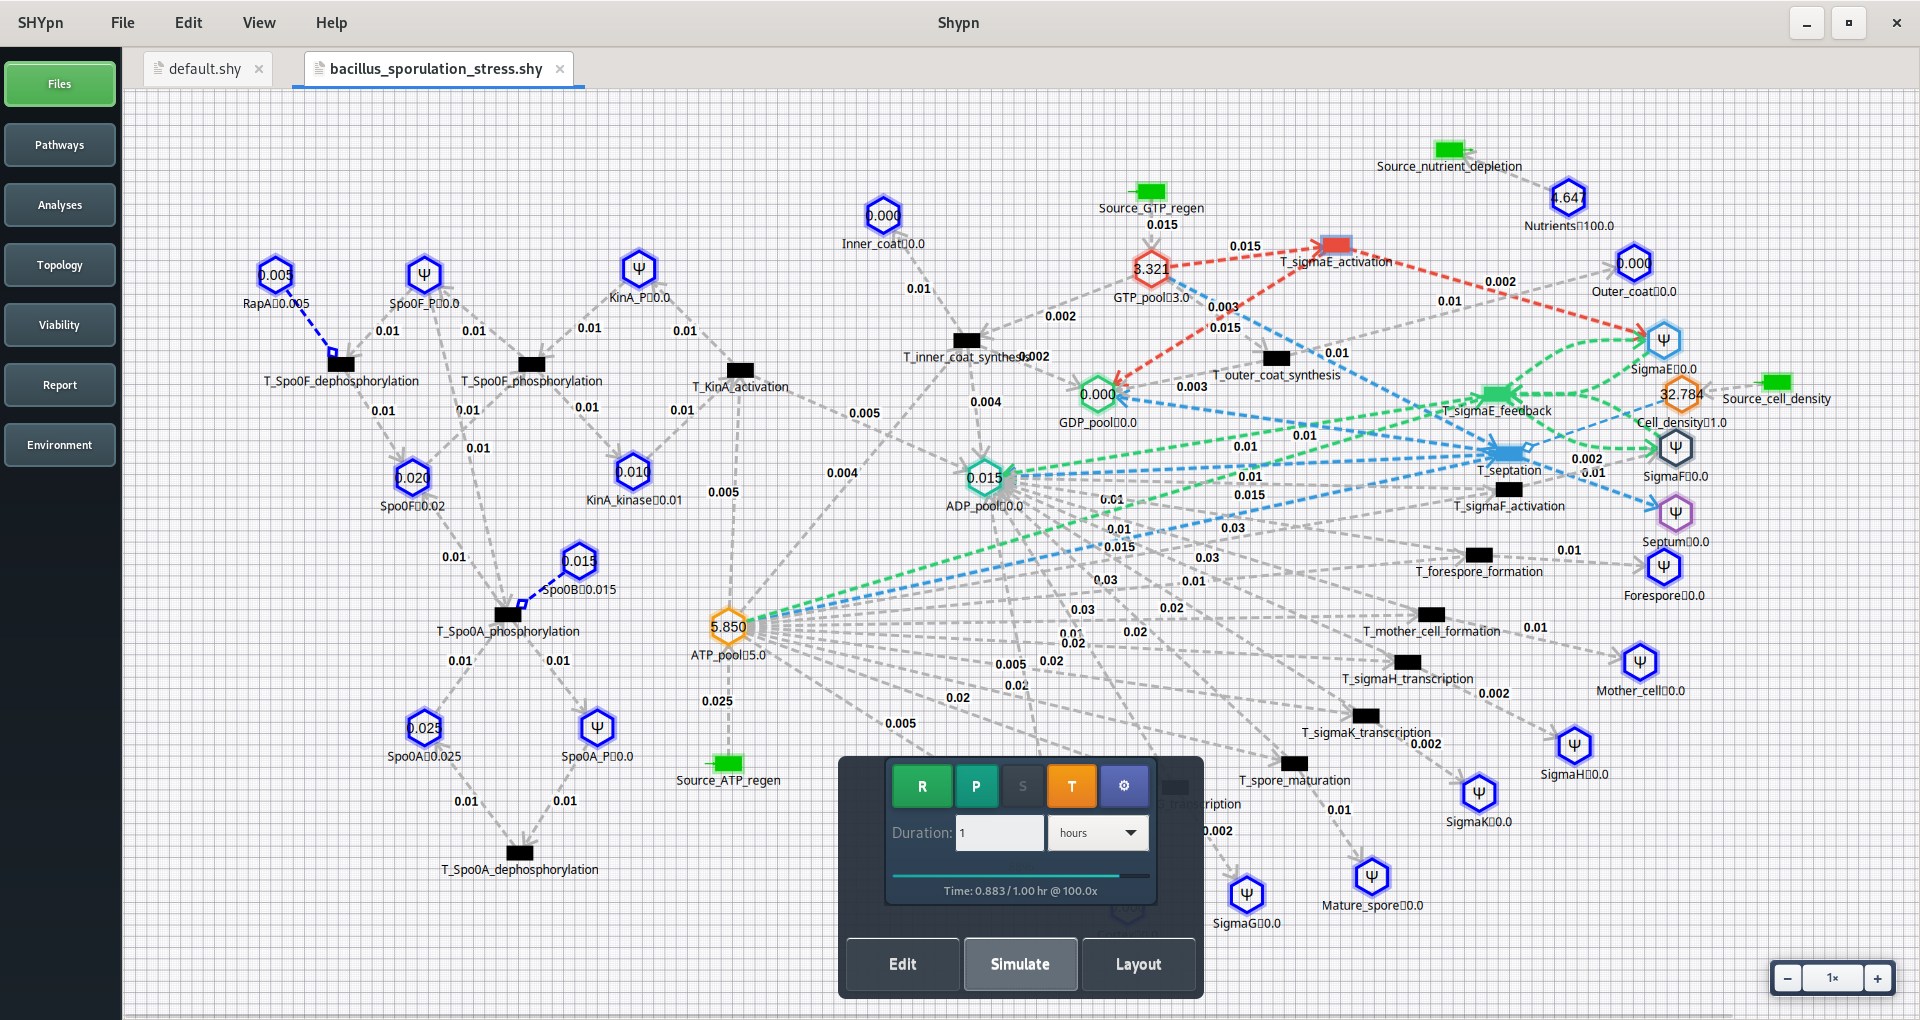
\includegraphics[width=\textwidth]{figures/Panels_SHYpn.png}
\caption{Fachada principal da SHYpn e paleta de painéis: cada painel
encapsula um contexto computacional persistente — construção de modelo,
simulação dinâmica, análise topológica, verificação de viabilidade e
geração de relatórios — permitindo navegação não linear entre fases
do fluxo de trabalho.}
\label{fig:panels-shypn}
\end{figure}

A SHYpn implementa uma \textbf{arquitetura multi-painel de documentos
persistentes} inspirada em ambientes de desenvolvimento integrado modernos
como Visual Studio Code, onde painéis especializados organizam a funcionalidade
por fase do fluxo de trabalho.

Cada painel funciona como um contexto computacional persistente com estado
independente.
O \textbf{Painel de Arquivos} (\textit{Explorer}) gerencia exclusivamente o
sistema de arquivos do projeto: árvore de diretórios, navegação
(avançar, retroceder, raiz), criação e abertura de projetos, e operações de
persistência (salvar, salvar como).
A \textbf{Tela de Modelagem} (\textit{Canvas}) é a superfície gráfica sobre
a qual o pesquisador constrói e edita o modelo: posiciona lugares e
transições, traça arcos, edita propriedades de cada objeto via diálogos
contextuais (marcação inicial, tipo de transição, constantes cinéticas,
designação de lugares de sinal $\Psi \subset P$) e instancia parâmetros
diretamente nos objetos do modelo.
O \textbf{Painel de Operações de Vias} (\textit{Pathway Operations})
constitui o centro de importação e enriquecimento paramétrico, reunindo
oito categorias: importação de vias KEGG (com conversão automática para
rede de Petri), importação de modelos SBML/BioModels, importação de modelos
genômicos BiGG, enriquecimento cinético via BRENDA (consulta por número EC
com seleção manual de parâmetros), enriquecimento via SABIO-RK (base pública
sem autenticação), inferência heurística de parâmetros baseada em tipo de
transição, histórico de enriquecimentos com rastreabilidade e avaliação, e
configuração termodinâmica universal.
A partir deste painel, modelos de fontes curadas são importados e traduzidos
diretamente para o formalismo SHPN; modelos que carecem de parâmetros cinéticos
podem ser inspecionados e enriquecidos consultando valores do BRENDA e SABIO-RK,
com edição interativa dos parâmetros selecionados.
A Figura~\ref{fig:e-coli-core} exemplifica a importação via Painel de
Operações de Vias: o modelo metabólico central de \textit{E.~coli}
(\textit{e\_coli\_core}) foi importado diretamente do repositório BiGG,
traduzido para rede de Petri e carregado na Tela de Modelagem para edição.

\begin{figure}[htbp]
\centering
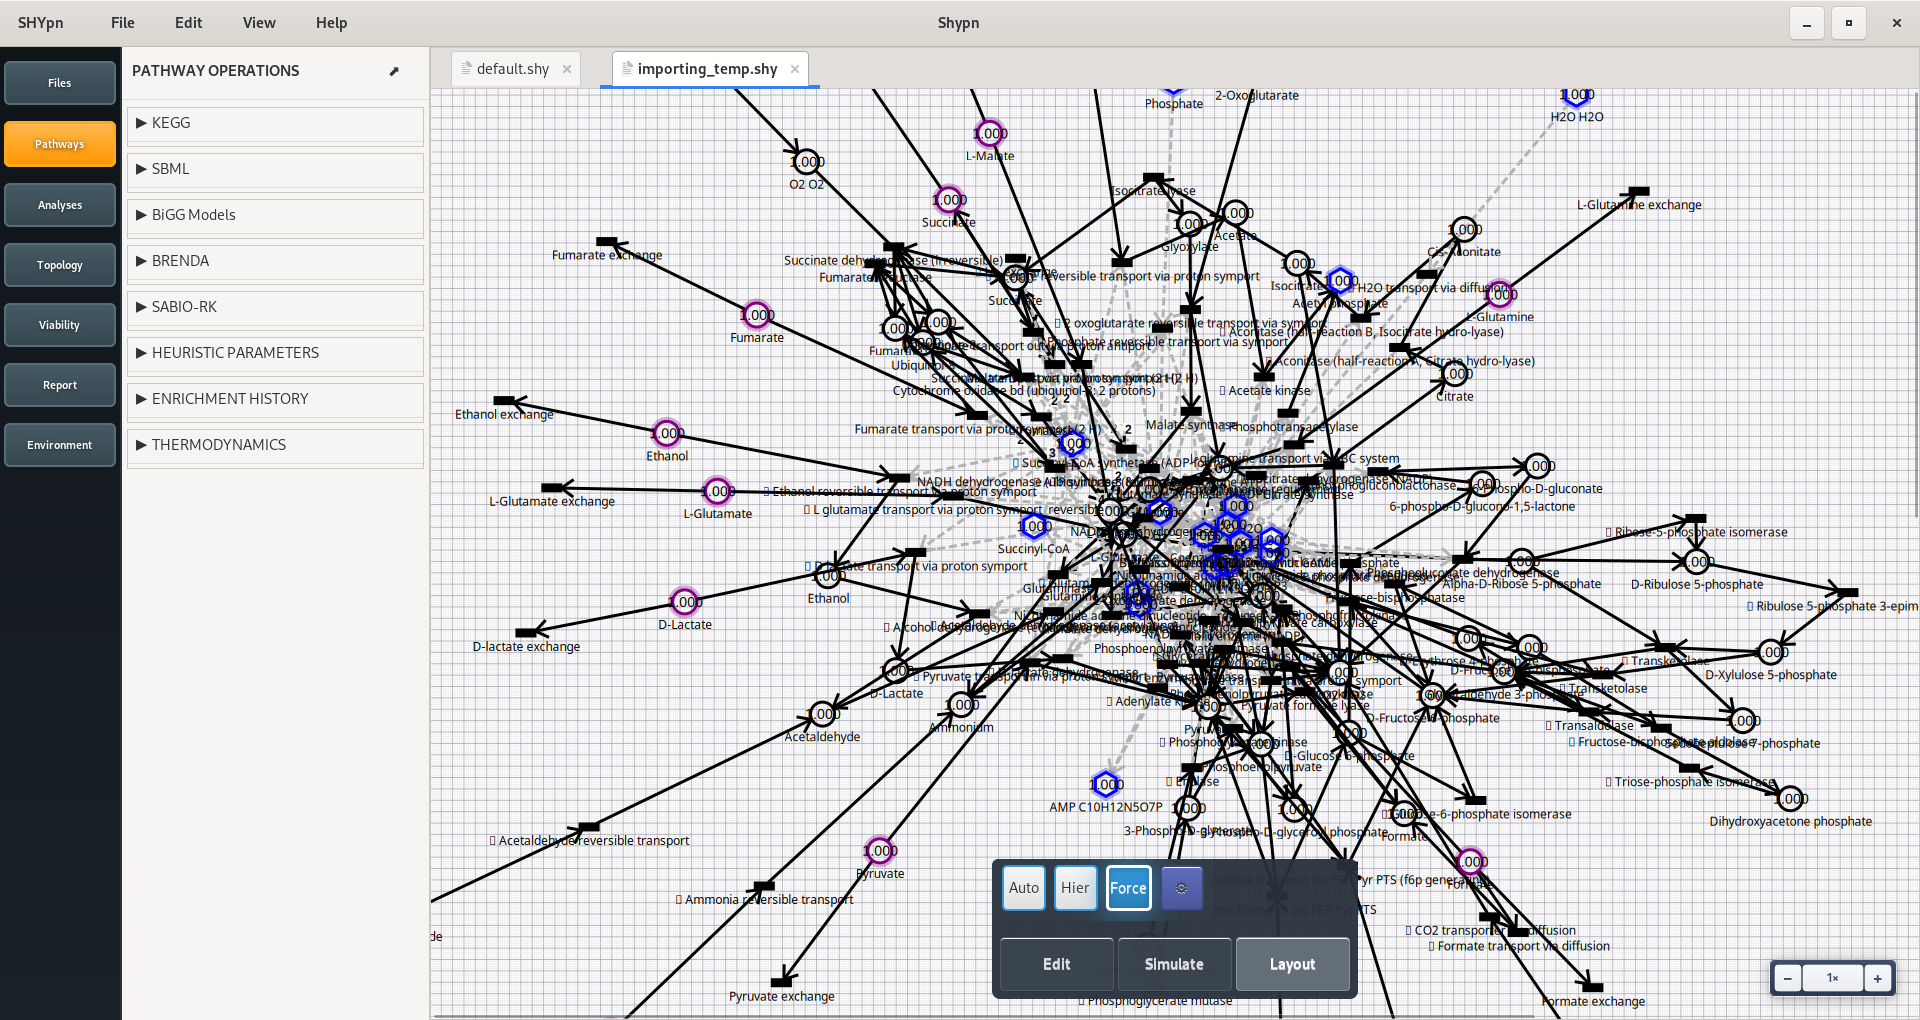
\includegraphics[width=\textwidth]{figures/e_coli_core.png}
\caption{Importação do modelo \textit{e\_coli\_core} a partir do
repositório BiGG via Painel de Operações de Vias: a SHYpn recupera
automaticamente a topologia SBML, converte para rede de Petri e
carrega o modelo na Tela de Modelagem para edição e simulação.}
\label{fig:e-coli-core}
\end{figure}

O \textbf{Painel de Análise} mantém o estado de simulação dinâmica com
atualização de gráficos de trajetória a 10~Hz, automação de varredura de
parâmetros e gerenciamento de réplicas estocásticas.
O \textbf{Painel de Topologia} calcula propriedades estruturais da rede —
P-invariantes representando leis de conservação, T-invariantes enumerando ciclos
de reação, análise do grafo regulatório revelando \textit{alças de retroalimentação},
\textit{hubs} e coeficientes de agrupamento, além de verificação de
vivacidade e limitação.
O \textbf{Painel de Viabilidade} isola a análise de sub-rede para investigação
focada: detecta componentes faltantes (substratos, catalisadores, produtos),
tenta verificar balanço elementar por consulta ChEBI ao nome dos compostos
--- quando a resolução é bem-sucedida --- e propõe correções estruturais
com capacidade de desfazer.
O \textbf{Painel de Relatório} sintetiza conteúdo de todos os painéis em
documentação pronta para publicação — tabelas de estrutura de modelo,
parâmetros, resultados de simulação, propriedades topológicas e registros de
correções de viabilidade, com exportação em PDF, Excel, JSON e Markdown.

\subsection{Sincronização entre Painéis}

Os painéis mantêm consistência por sincronização automática de dados.
Modificar a estrutura da rede na Tela de Modelagem desencadeia atualizações
imediatas: o Painel de Análise invalida resultados de simulação obsoletos, o
Painel de Topologia invalida P-invariantes em cache, o Painel de Viabilidade
atualiza a análise de dependências e o Painel de Relatório atualiza as
estatísticas de estrutura do modelo.
A sincronização respeita o custo computacional: atualizações leves (contagem de
lugares/transições) ocorrem imediatamente; recomputações custosas (P-invariantes,
análise de grafo regulatório) ocorrem sob demanda, sinalizadas por emblemas
visuais ``Desatualizado'' que solicitam atualização explícita.
Essa sincronização elimina uma fonte de erro comum na biologia computacional —
modelos modificados sem atualização da documentação correspondente.

\section{Painéis: Suporte ao Fluxo de Trabalho Biológico}
\label{sec:paineis}

\subsection{Painel de Arquivos: Gestão de Arquivos do Projeto}

A Figura~\ref{fig:explorer-panel} mostra o Painel de Arquivos aberto na
SHYpn, com a árvore de diretórios do projeto e os controles de navegação.

\begin{figure}[htbp]
\centering
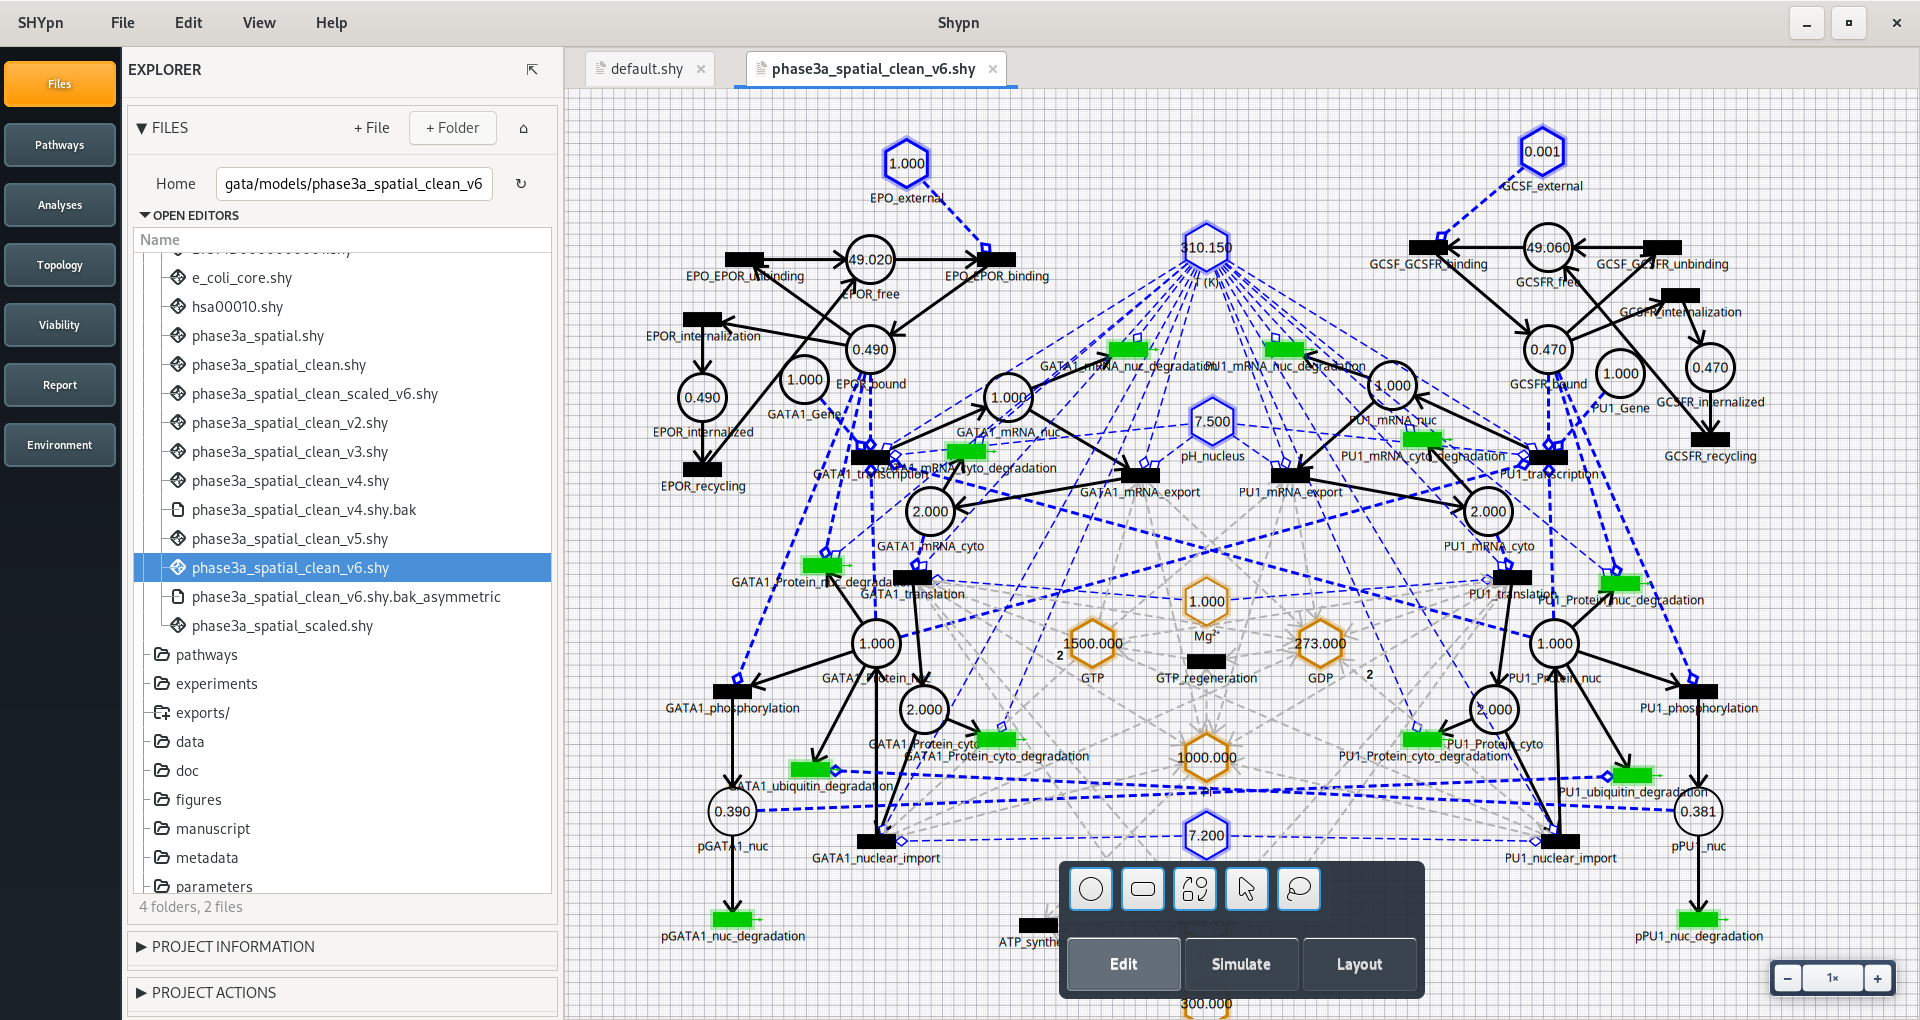
\includegraphics[width=\textwidth]{figures/explorer.png}
\caption{Painel de Arquivos (\textit{Explorer}) da SHYpn: árvore de
diretórios do projeto com navegação hierárquica, controles de
persistência (novo, abrir, salvar) e gestão de projetos.}
\label{fig:explorer-panel}
\end{figure}

O Painel de Arquivos (\textit{Explorer}) é exclusivamente dedicado à gestão
do sistema de arquivos do projeto.
Fornece uma árvore de diretórios com navegação completa (avançar, retroceder,
subir nível, voltar à raiz do projeto), barra de ferramentas para operações de
arquivo (novo, abrir, salvar, salvar como) e ações de projeto (novo projeto,
abrir projeto, configurações).
O Painel de Arquivos \emph{não} intervém na edição do modelo nem na atribuição
de parâmetros --- essas responsabilidades pertencem à Tela de Modelagem e ao
Painel de Operações de Vias, respectivamente.

\subsection{Tela de Modelagem: Desenho e Parametrização do Modelo}

A Tela de Modelagem (\textit{Canvas}) é a superfície gráfica central da SHYpn,
sobre a qual o pesquisador constrói visualmente a rede de Petri e instancia
parâmetros nos objetos do modelo.
A tela suporta documentos múltiplos com abas independentes, cada uma mantendo
um \texttt{ModelCanvasManager} com coleções isoladas de lugares, transições e
arcos, estado de zoom/pan e grade adaptativa.

A construção do modelo opera por interação direta: o pesquisador seleciona a
ferramenta adequada na paleta (\textit{SwissKnifePalette}) e clica na tela para
posicionar lugares e transições, ou arrasta entre objetos para traçar arcos.
Diálogos contextuais (acessados por duplo clique ou menu de contexto) permitem
editar cada propriedade: marcação inicial~$M_0(p)$, tipo de transição
(contínua, estocástica, temporizada, imediata), constantes cinéticas
($K_m$, $V_{\text{max}}$), peso de arcos e designação de lugares de sinal
($\Psi \subset P$).
A distinção visual emprega bordas azuis (lugares de sinal) \textit{versus} bordas
pretas (lugares normais), correspondendo ao modelo de validação do
\textit{Bacillus} (Capítulo~\ref{ch:validacao-bacillus}), onde os lugares de
sinal designados foram suficientes para produzir o limiar emergente de decisão.

A atribuição de parâmetros rastreia a proveniência por cor: valores padrão
importados do KEGG (células cinzas), medidas experimentais enriquecidas pelo
BRENDA (células azuis) e edições manuais do usuário (células laranja), permitindo
avaliar a confiança paramétrica --- modelos com 90\% de enriquecimento BRENDA
possuem embasamento empírico mais robusto.

\subsection{Painel de Operações de Vias: Importação e Enriquecimento}

O Painel de Operações de Vias (\textit{Pathway Operations}) constitui o centro
de importação de modelos e enriquecimento paramétrico da SHYpn, reunindo oito
categorias funcionais numa interface unificada.

\textbf{Importação de modelos curados.}
Três categorias permitem importar modelos diretamente de bases de dados curadas,
com conversão automática para o formalismo SHPN:
(i)~\textbf{KEGG} --- o usuário fornece um identificador de via (ex.: hsa00010)
e a SHYpn busca os dados KGML, analisa a via e converte-a em rede de Petri
com layout preservado;
(ii)~\textbf{SBML/BioModels} --- importação de arquivos SBML locais ou busca
remota no repositório BioModels, com detecção automática de compartimentos e
pós-processamento de layout;
(iii)~\textbf{BiGG} --- navegação e importação de modelos genômicos de escala
genômica a partir do repositório BiGG, com classificação automática de
lugares de sinal.

\paragraph{Mapeamento SBML $\to$ 13-tupla + grafo de parâmetros.}
A importação SBML não é mera tradução sintática: a SHYpn classifica os
elementos do documento SBML nas categorias semânticas do formalismo SHPN
(Capítulo~\ref{ch:shpn}, Tabela~\ref{tab:decisoes-modelador}). Cada
\texttt{species} torna-se um lugar $p \in P$, com a anotação
\texttt{compartment} preservada como metadado e usada pelo
\textit{compartment-module service} para induzir a partição em módulos.
Cada \texttt{reaction} torna-se uma transição $t \in T$ com tipo $\Phi(t)$
derivado da \textit{kinetic law} (contínua quando há lei explícita,
estocástica quando o anotador SBO sinaliza Hill ou Mass Action discreto).
Os \texttt{reactants} e \texttt{products} mapeiam para arcos $F$ com pesos
estequiométricos; os \texttt{modifiers} requerem desambiguação semântica:
ausentes da lei cinética ou anotados como catálise são convertidos em
arcos de teste $F_t$; presentes na lei com termo de Hill ou cooperatividade
notacionalmente compatível com $\Gamma$ são promovidos a arcos de fluxo de
sinal $F_s$ e o lugar correspondente é anexado a $\Psi$.

Os \texttt{parameters} globais e os \texttt{initial assignments} do SBML
não entram na rede-objeto: são instanciados como \textbf{lugares de
parâmetro} ($\Box$, \texttt{is\_parameter\_place=true}) no \emph{grafo de
parâmetros} separado, e os \texttt{events} do SBML preservam-se como
eventos do plano experimental (Capítulo~\ref{ch:shpn},
Seção~\ref{sec:planejamento-experimental}). Essa separação
rede-objeto / plano experimental --- ausente no documento SBML original
--- materializa-se durante a importação e é condição necessária para que o
modelo importado se beneficie das varreduras paramétricas e da
proveniência hierárquica descritas adiante.
Metadados curatoriais (anotações MIRIAM, referências cruzadas a ChEBI, KEGG,
UniProt, e o próprio identificador BioModels do documento de origem) são
retidos como propriedades por objeto, permitindo rastrear cada elemento
da rede SHPN até sua origem no SBML curado.

\textbf{Enriquecimento paramétrico.}
Modelos importados frequentemente carecem de constantes cinéticas.
Três categorias resolvem essa lacuna:
(i)~\textbf{BRENDA} --- após autenticação, o pesquisador consulta o BRENDA por
número EC ou nome de reação, visualiza os parâmetros cinéticos disponíveis
($K_m$, $k_{\text{cat}}$, $V_{\text{max}}$) e seleciona manualmente quais
aplicar ao modelo;
(ii)~\textbf{SABIO-RK} --- base de dados pública (sem autenticação) com o
mesmo fluxo de consulta e seleção manual;
(iii)~\textbf{Inferência Heurística} --- inferência inteligente de parâmetros
com base no tipo de transição (contínua, estocástica, temporizada, imediata)
e contexto biológico, aprendendo do histórico de enriquecimentos anteriores.

A categoria \textbf{Histórico de Enriquecimentos} permite rastrear, avaliar e
desfazer aplicações de parâmetros, garantindo rastreabilidade completa.
A categoria \textbf{Termodinâmica} configura as definições de validação
termodinâmica universal e mapeamento de compostos.

\subsection{Painel de Análise: Simulação Dinâmica}

O Painel de Análise expõe controle de simulação e visualização de trajetórias
em tempo real.
A Figura~\ref{fig:dynamic-analysis} ilustra a interface desse painel,
com os controles de simulação e a visualização de trajetórias dinâmicas.

\begin{figure}[htbp]
\centering
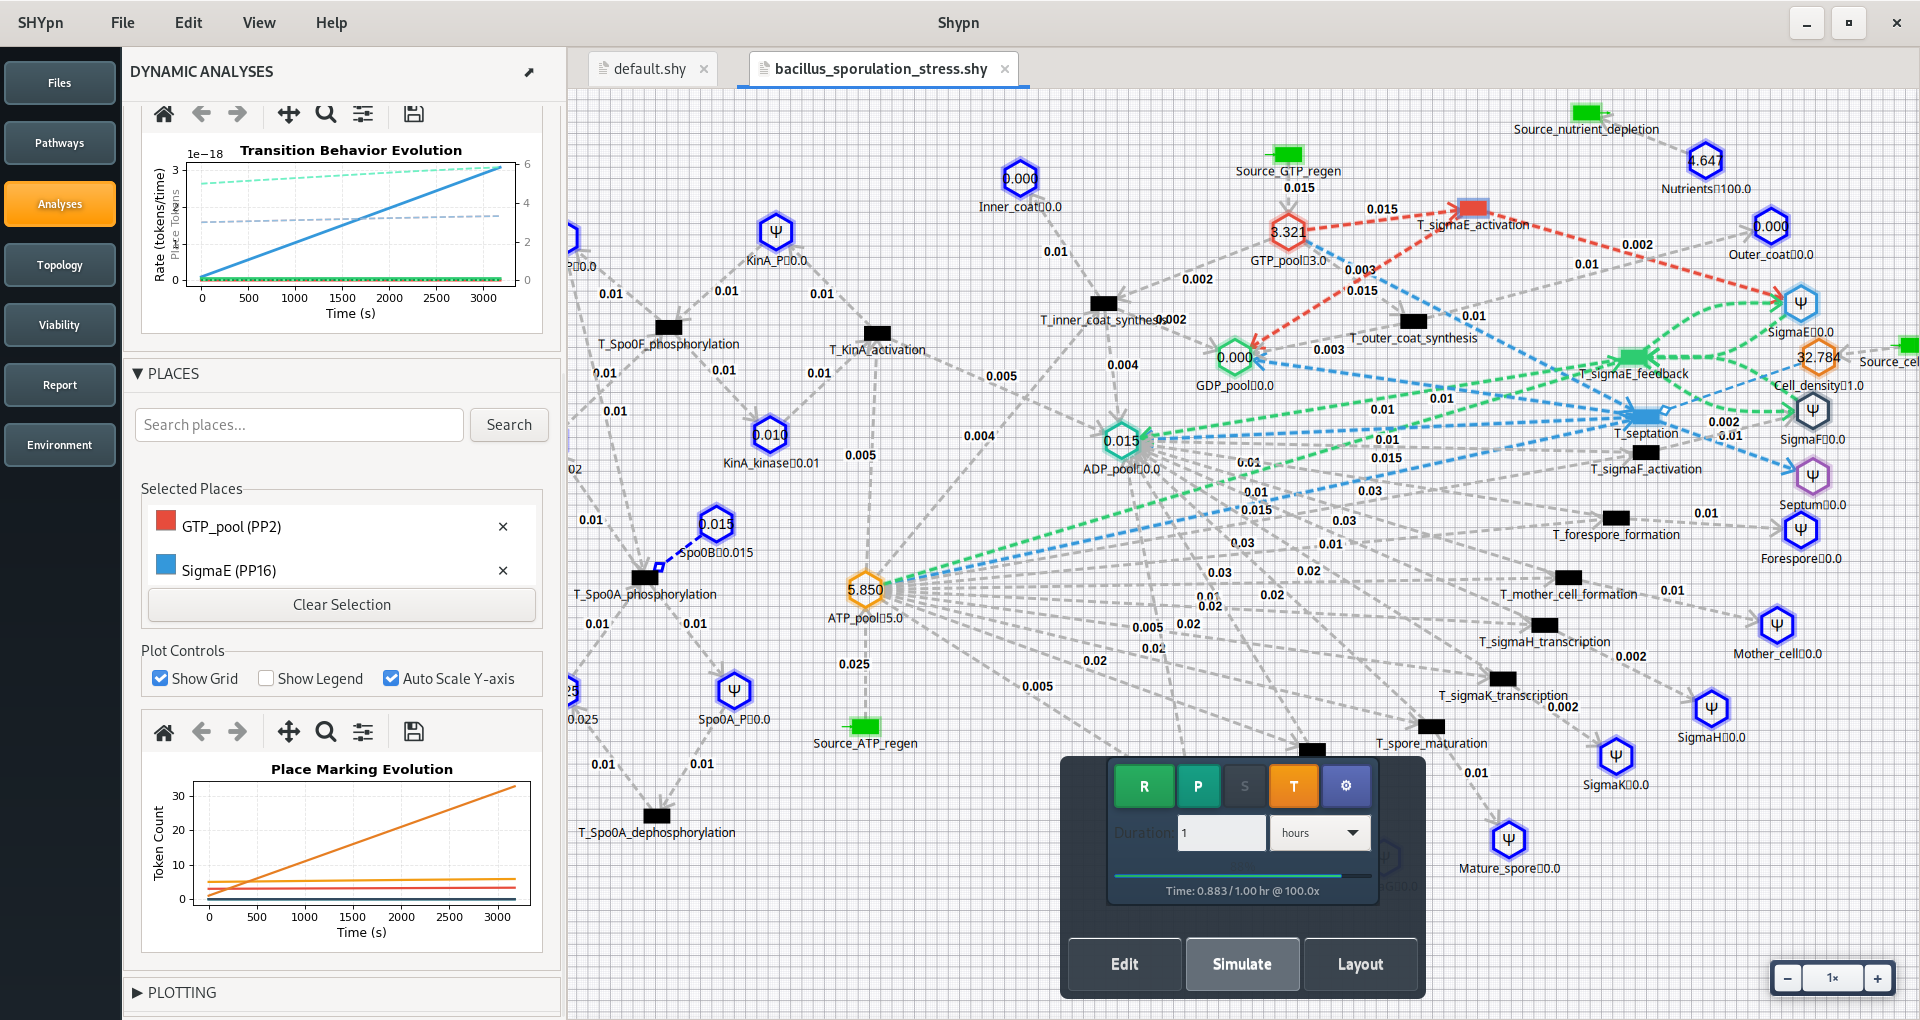
\includegraphics[width=\textwidth]{figures/Dynamic_analysis.png}
\caption{Painel de Análise Dinâmica da SHYpn: controles de simulação
(duração, passo, solver), gráficos de trajetória atualizados em tempo
real e sobreposições de limiar para identificação de regimes regulatórios.}
\label{fig:dynamic-analysis}
\end{figure}

Pesquisadores configuram parâmetros de simulação (duração, passo de tempo,
seleção de solver de EDO, contagem de réplicas estocásticas), iniciam a execução
e observam a evolução de marcação $M(p, t)$ por gráficos atualizados
dinamicamente.
Sobreposições de limiar marcam concentrações biologicamente significativas
($[\sigma^H] = \theta_{\sigma H} \approx 1{,}60\,\mu$M, $[\text{Spo0A}{\sim}\text{P}] = 20\ \mu$M),
alertando quando simulações entram em regimes regulatórios preditos.
A automação de varredura de parâmetros explora espaços multidimensionais:
variando $K_m$ de 0,01 a 1~mM (10 etapas logarítmicas) com $V_{\text{max}}$
de 1 a 10~mM/s (10 etapas lineares) gera uma grade 10$\times$10 de simulações,
com visualização em mapa de calor revelando relações compensatórias.
O modo de simulação estocástica executa 100 ou mais réplicas com sementes
aleatórias independentes, quantificando o ruído intrínseco: o coeficiente de
variação CV~=~$\sigma/\mu$ revelou variabilidade celular de $\sim\!15\%$ na
ativação do fator sigma durante a validação da esporulação do
\textit{Bacillus}, compatível com distribuições experimentais.

\subsection{Painel de Topologia: Análise Estrutural}

A Figura~\ref{fig:topology-panel} mostra o Painel de Topologia durante a
execução de análises estruturais e comportamentais do modelo GATA, com os
resultados de P-invariantes, T-invariantes e propriedades do grafo regulatório.

\begin{figure}[htbp]
\centering
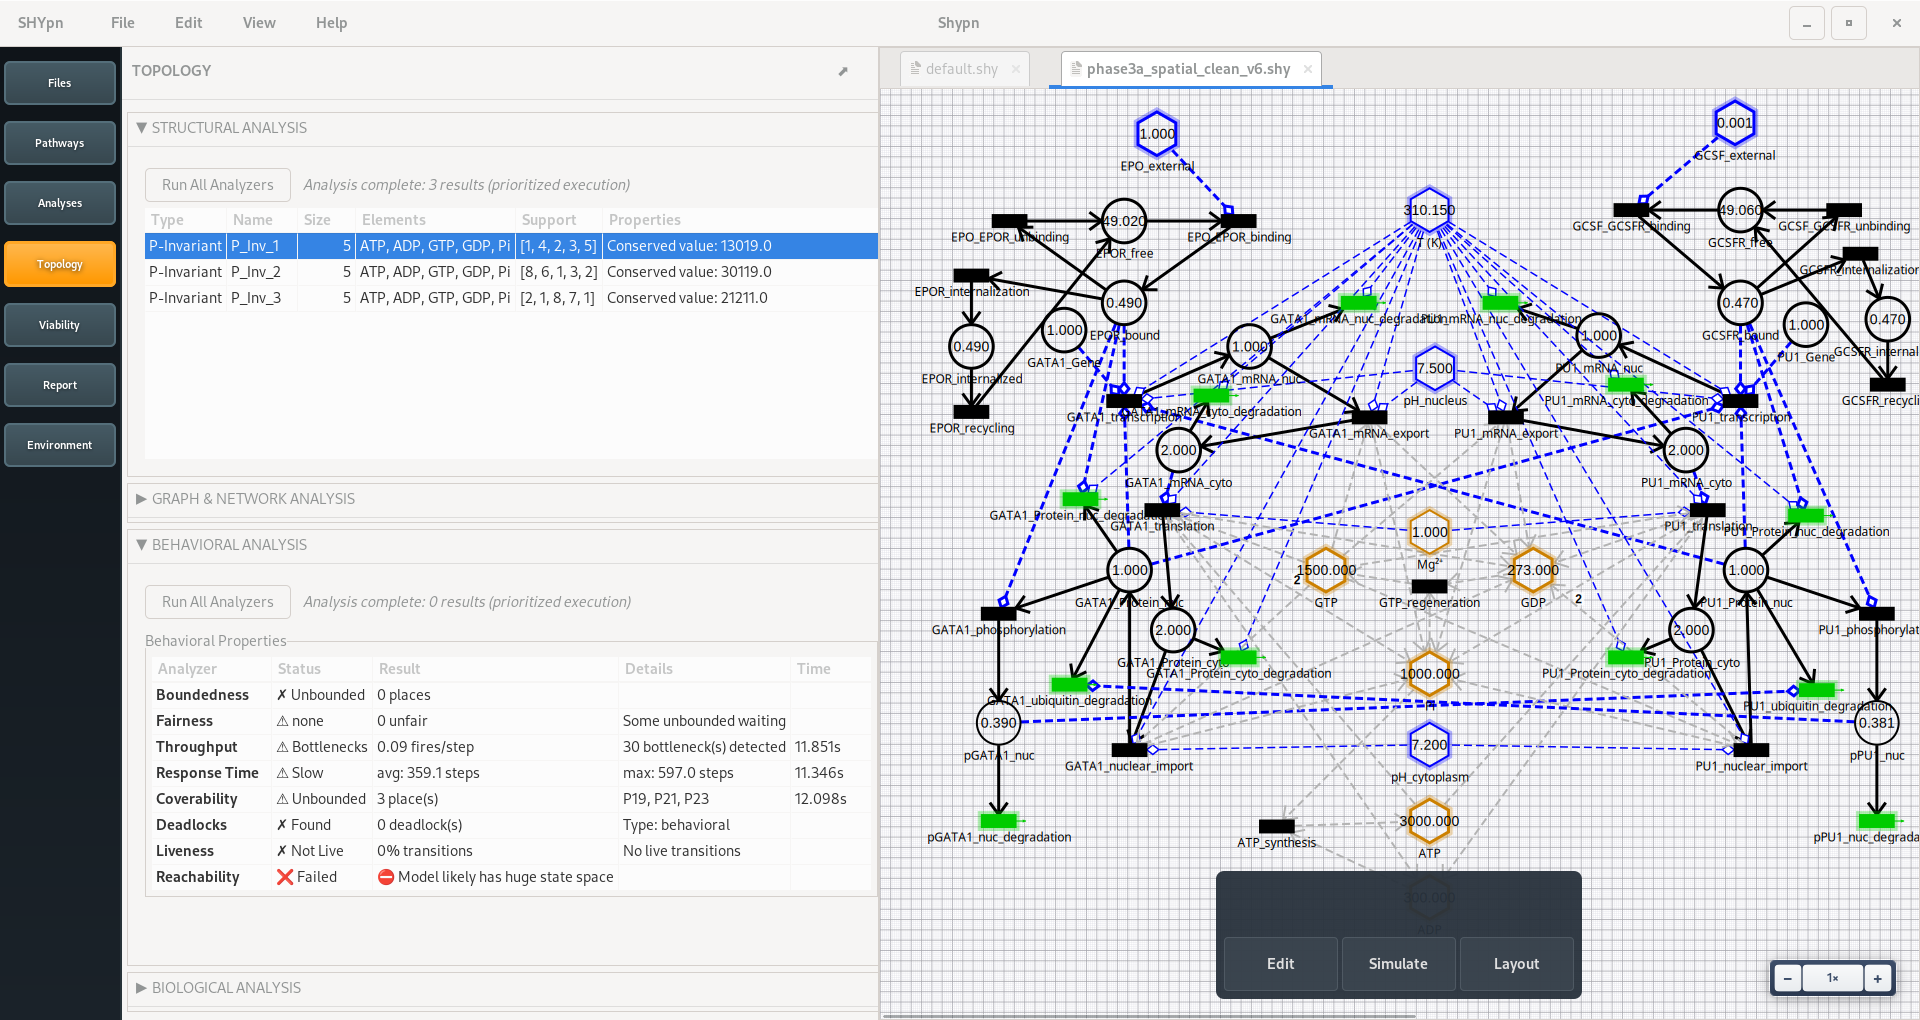
\includegraphics[width=\textwidth]{figures/Topology.png}
\caption{Painel de Topologia da SHYpn executando análise estrutural e
comportamental do modelo GATA: a interface exibe P-invariantes (leis de
conservação), T-invariantes (ciclos de reação) e propriedades do grafo
regulatório, permitindo validação da conectividade da rede antes da
simulação dinâmica.}
\label{fig:topology-panel}
\end{figure}

O Painel de Topologia calcula propriedades de rede independentes de parâmetros
cinéticos, revelando capacidades e restrições inerentes à conectividade da rede.
A \textbf{análise estrutural} identifica P-invariantes (leis de conservação como
ATP~+~ADP~+~AMP~=~const) e T-invariantes (ciclos de reação como o ciclo de
glicose~6-fosfato).
A \textbf{análise de grafos} constrói grafos regulatórios a partir de arcos de
teste e de inibição, detectando \textit{alças} de retroalimentação positivas
(que impulsionam biestabilidade) e negativos (que permitem oscilações), além
de classificar hubs como ATP, NAD$^+$ e CoA.
A \textbf{análise de dependências} aplica a classificação de independência fraca
do Capítulo~\ref{ch:shpn} para particionar pares de transições em
independentes (lugares de entrada disjuntos), fracamente dependentes
(entradas somente leitura compartilhadas) e fortemente acoplados (operações de
escrita conflitantes), habilitando simulação paralela com \textit{speedup}
de 1,9$\times$ para o modelo do \textit{Bacillus} em 4 núcleos.
As leis de conservação são verificadas numericamente
após cada passo da simulação, com tolerância $\| C^T \cdot M(t) \| < 10^{-6}$.

\subsection{Painel de Viabilidade: Refinamento Inteligente}

A Figura~\ref{fig:viability-panel} mostra o Painel de Viabilidade durante
uma varredura por planejamento fatorial, onde combinações de parâmetros são
exploradas sistematicamente para avaliar a robustez do modelo.

\begin{figure}[htbp]
\centering
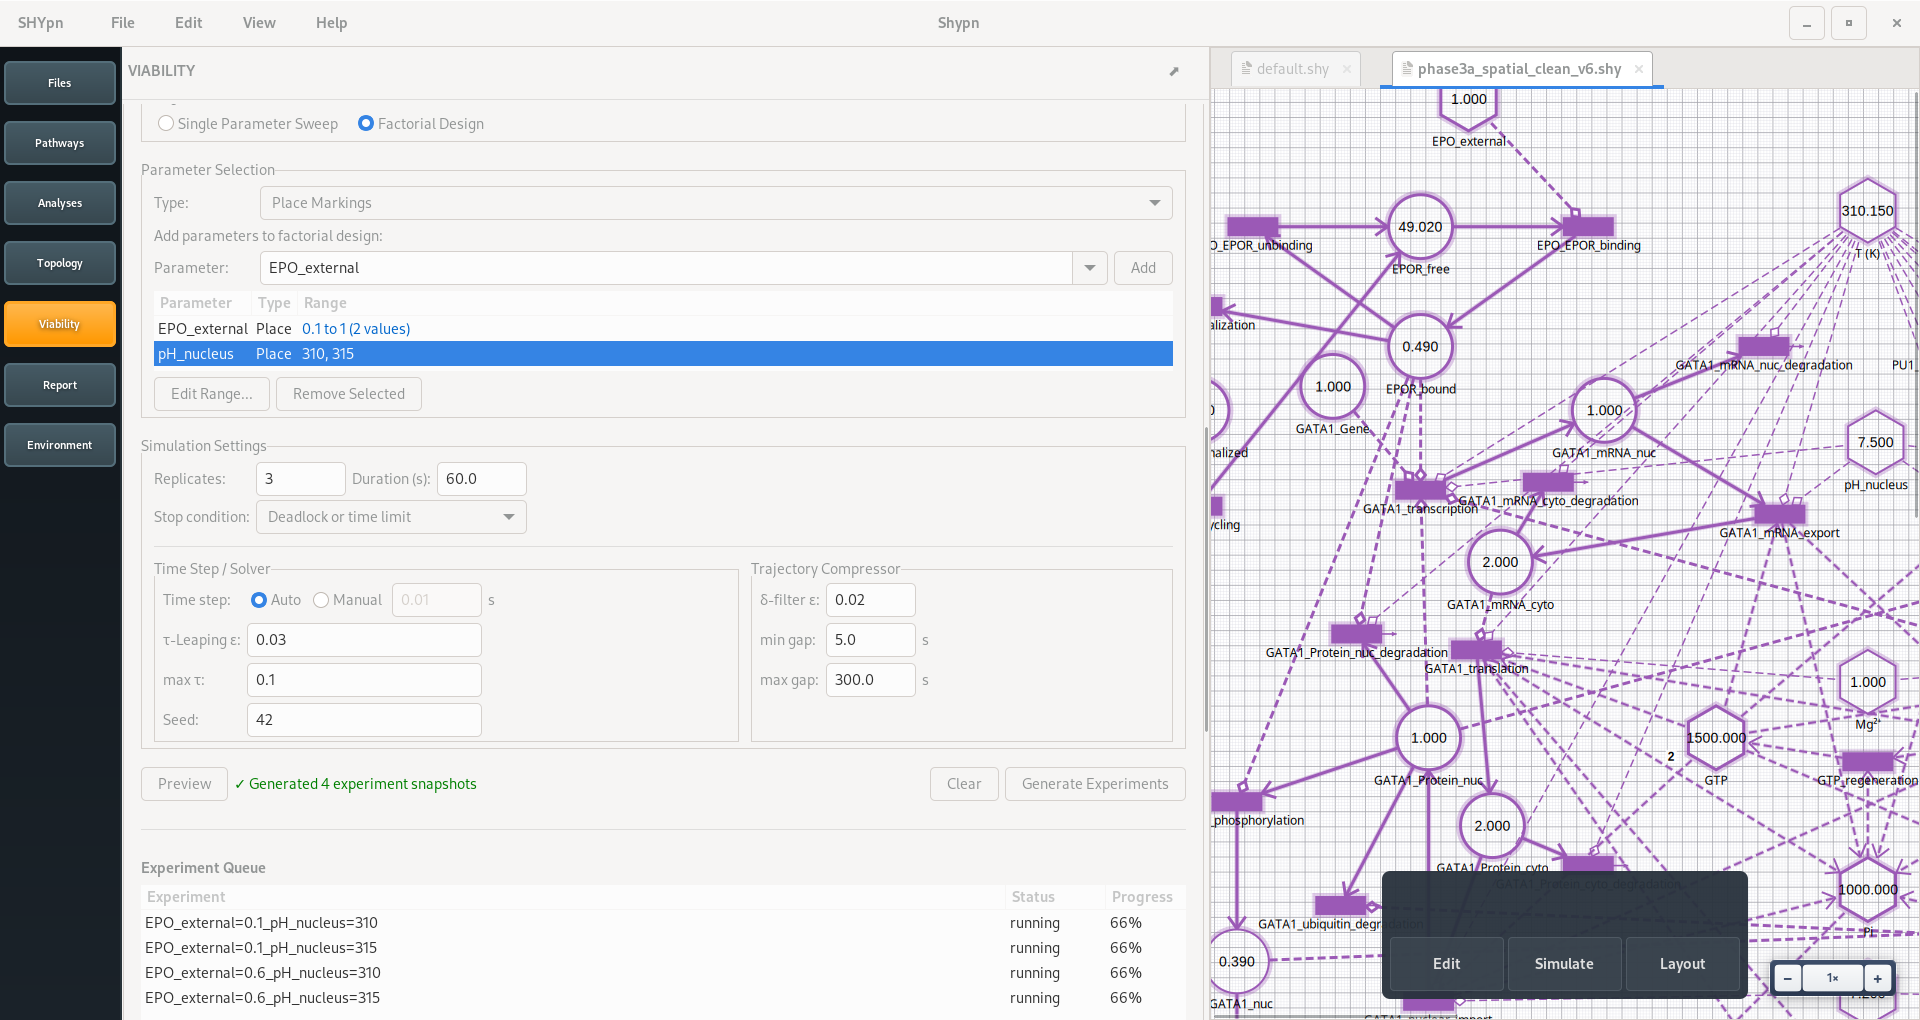
\includegraphics[width=\textwidth]{figures/Viablity.png}
\caption{Painel de Viabilidade da SHYpn executando uma varredura por
planejamento fatorial: os analisadores especializados verificam
dependências, disponibilidade de substratos e balanço elementar,
enquanto a varredura paramétrica identifica regiões de operação viável
do modelo.}
\label{fig:viability-panel}
\end{figure}

Modelos biológicos crescem incrementalmente; o rastreamento manual de
dependências falha para redes com mais de cerca de 20 componentes.
O Painel de Viabilidade automatiza a detecção de dependências por quatro
analisadores especializados.
O \textbf{Analisador de Localidade} verifica a disponibilidade de substratos,
presença de catalisadores e consumo de produtos.
O \textbf{Analisador de Dependências} consulta bases de conhecimento
bioquímico — quinases requerem ATP, transcrição necessita nucleotídeos,
fosforilação libera ADP — para detectar lógica regulatória ausente.
O \textbf{Analisador de Fronteira} examina lugares de oferta infinita
conferindo plausibilidade termodinâmica.
O \textbf{Analisador de Conservação} tenta verificar o balanço elementar
consultando o ChEBI pelo nome de cada composto; nos casos em que a
resolução é unívoca, o módulo exige conservação de C, H, O, N e P.
A heterogeneidade de notações de nomes limita a cobertura, e não há
interface para entrada manual de fórmulas.
O fluxo de 22 transições do modelo do \textit{Bacillus} exigiu dezenas de
iterações de refinamento; o Painel de Viabilidade identificou
arcos de teste faltantes ao longo desse processo.

\section{Arquitetura Dual do Motor de Simulação}
\label{sec:motores-simulacao}

O Capítulo~\ref{ch:shpn} define a evolução da marcação por regra
de disparo: $M(t+\Delta t) = M(t) + C \cdot \vec{v}(t)$, onde~$C$ é a matriz
estequiométrica e $\vec{v}(t)$ o vetor de taxas de disparo.
Essa abstração oculta complexidade de implementação significativa; a SHYpn a
aborda com uma \textbf{arquitetura dual} que suporta dinâmicas contínua (baseada
em EDO) e estocástica (Gillespie) com escalonamento hierárquico unificado.

\subsection{Motor Contínuo: Integração de EDO}

Reações metabólicas operando em grandes populações moleculares exibem
dinâmicas determinísticas bem aproximadas por EDOs.
O motor contínuo executa cinco etapas coordenadas.

\textbf{Avaliação da função de taxa:} para cada transição $t \in T$, avalia-se
$r(t, M)$ com as leis cinéticas suportadas: ação de massa ($r = k \cdot \prod M(p)$),
Michaelis-Menten ($r = V_{\text{max}} \cdot M(S) / (K_m + M(S))$), Hill
($r = V_{\text{max}} \cdot M(S)^n / (K_d^n + M(S)^n)$) e expressões Python
personalizadas.

\textbf{Gateamento por limiar via $\Gamma$:} para cada lugar de sinal
$p_s \in \Psi$ com parâmetro termodinâmico associado, computa-se o limiar
efetivo $\theta_{\text{eff}}(p_s) = K \cdot (\varepsilon /
(1 - \varepsilon))^{1/n}$ e a função indicadora
$\Theta(p_s, M) = \mathbf{1}[M(p_s) \geq \theta_{\text{eff}}(p_s)]$.
Multiplica-se a taxa de transição pelo produto dessas funções indicadoras:
$v(t) = r(t, M) \cdot \prod_{(p_s,t) \in F_s} \Theta(p_s, M)$,
implementando o predicado de habilitação da
Definição~\ref{def:habilitacao} do Capítulo~\ref{ch:shpn}.

\textbf{Preempção hierárquica:} transições são particionadas por camada, computa-se
a camada mínima ativa $\lambda_{\min}$, e todas as transições com
$\lambda(t) > \lambda_{\min}$ são desabilitadas com $v(t) = 0$, implementando
a preempção de camada (Teorema~\ref{thm:preempcao}).

\textbf{Integração do sistema de EDO:} monta-se $dM/dt = C \cdot \vec{v}(M, t)$
e integra-se com Runge--Kutta de 4ª ordem (RK4) de passo fixo, acoplado
à amostragem $\tau$-leaping (Subseção~\ref{subsec:motor-estocastico})
por divisão de operador (\emph{operator splitting}) por passo de tempo:
fluxo contínuo $\to$ disparos estocásticos $\to$ finalização.

\textbf{Verificação de leis de conservação:} após cada passo de tempo,
verifica-se $\|C^T \cdot M(t)\| < 10^{-6}$; violações acionam avisos que
indicam erros estequiométricos ou instabilidade numérica.
Este motor simula o modelo do \textit{Bacillus} (40~lugares e
36~transições --- ver
Capítulo~\ref{ch:validacao-bacillus}) em tempo de parede inferior a 5~s
(21.600~s de tempo biológico).

\subsection{Motor Estocástico: $\tau$-leaping}
\label{subsec:motor-estocastico}

Espécies regulatórias com baixo número de cópias ($\sim\!100$ moléculas de
fatores de transcrição, $\sim\!10$ moléculas de mRNA) exibem flutuações
estocásticas onde a aproximação determinística por EDO falha.
O motor estocástico implementa o algoritmo \textbf{$\tau$-leaping}
(\textcite{Gillespie2001}), uma aproximação acelerada do SSA exato de
\textcite{Gillespie1977} --- cuja variante eficiente por grafo de dependências
é o método de \textcite{Gibson2000} --- adaptada para redes de Petri hierárquicas: em
cada passo $\tau$, o número de disparos de cada transição é amostrado de
uma distribuição de Poisson com média $a(t,M)\cdot\tau$, em vez de
selecionar uma única reação por evento como no SSA exato.
Reações reversíveis acopladas (forma $A \rightleftharpoons B$ detectadas
por convenção de nomenclatura $k_f / k_r$) são amostradas pelo estimador
Skellam (Poisson direta menos Poisson reversa) para correto tratamento
do balanço detalhado.

Para cada transição $t$, a propensão é
\[
  a(t, M) = r(t, M) \cdot \prod_{p \in \bullet t} \binom{M(p)}{W((p,t))},
\]
levando em conta combinações moleculares discretas.
O gateamento por limiar e a preempção hierárquica são aplicados de forma
idêntica ao motor contínuo, zerando $a(t)$ para transições desabilitadas.
A cada passo, o tamanho $\tau$ é selecionado adaptativamente de modo a
limitar a variação relativa esperada de cada espécie a uma fração
configurável (controle de erro $\varepsilon_\tau$); para cada transição,
amostra-se o número de disparos $k_t \sim \mathrm{Poisson}(a(t,M)\cdot\tau)$
e a marcação é atualizada por $M' = M + \sum_t k_t \cdot C_t$, onde $C_t$ é
a coluna estequiométrica de $t$.
O modo híbrido trata modelos que misturam metabolismo contínuo (ATP e glicose
de alta cópia) com regulação discreta (fatores sigma de baixa cópia),
particionando automaticamente as transições em subconjuntos integrados por EDO
e amostrados por $\tau$-leaping com base nas marcações dos lugares, acoplando
os subsistemas por lugares compartilhados.
Um tipo \emph{adaptativo} adicional --- detalhe de implementação, não
primitivo do formalismo --- alterna automaticamente entre os modos contínuo
e estocástico por transição, com base no volume de compartimento e em um
limiar de número de cópias configurável.
A simulação estocástica do modelo do \textit{Bacillus} completou-se em 4,1~s
(réplica única); varreduras de parâmetros de 100 simulações em modo paralelo
(4 núcleos) finalizaram em 1,2~min (3,2$\times$ de \textit{speedup}).

\section{Qualidade de Implementação}
\label{sec:qualidade-implementacao}

\subsection{Pilha de Tecnologias}

A SHYpn utiliza Python~3.10+ para flexibilidade de domínio biológico com
desempenho por vetorização NumPy nos laços de avaliação de função de taxa
e, opcionalmente, por aceleração GPU via CuPy (\texttt{GPUHybridEngine},
backend CUDA~12.x para placas com suporte a precisão dupla);
GTK3 para arquitetura multi-janela com integração nativa de sistema
operacional e Matplotlib para gráficos de trajetória com qualidade de
publicação.
A integração com banco de dados emprega clientes de API REST consultando KEGG,
BRENDA e ChEBI com cache SQLite local que reduz requisições de rede e habilita
operação offline.
A persistência em JSON possibilita controle de versão Git, e contêineres Docker
que encapsulam o ambiente computacional completo garantem reprodutibilidade
bit-a-bit independentemente do sistema operacional do usuário.

\subsection{Métricas de Desempenho}

O modelo do \textit{Bacillus} (40~lugares e 36~transições) simula 6~h de
tempo biológico em tempo de parede inferior a 5~s no motor de EDO.
O Painel de Análise atualiza gráficos a 10~Hz durante a simulação sem atraso
perceptível, com buffers de trajetória armazenando 10.000 pontos temporais
($\sim\!12$~MB por modelo) e habilitando zoom e panorâmica dinâmicos.
O cálculo de P-invariantes (decomposição SVD de $C^T$) completa-se em menos de
1~s para o modelo do \textit{Bacillus} (matriz $40 \times 36$) e em 8,3~s para
redes de escala genômica (200 lugares $\times$ 150 transições).
O Painel de Viabilidade executa simulações de sub-rede (15 transições, 10 lugares)
em 0,3~s, habilitando ciclos interativos de refinamento de $\sim\!5$~s.
A pegada de memória do modelo do \textit{Bacillus} permanece dentro das
restrições de laptop, com escalonamento linear para redes de escala genômica.

\subsection{Garantia de Qualidade}

A cobertura de testes é de 87\% para os motores de simulação e de 68\% para
os componentes de interface, com 427 testes unitários verificando comportamento
individual de componentes: testes do motor de EDO comparam trajetórias simuladas
com soluções analíticas (decaimento exponencial, crescimento logístico), e
testes do motor de Gillespie verificam cálculos de propensão e distribuições de
amostragem de eventos.
Vinte e dois testes de integração executam fluxos completos — importação KEGG,
enriquecimento BRENDA, simulação, exportação de relatório — em exemplos de
validação (Capítulo~\ref{ch:validacao-bacillus}).
Asserções em tempo de execução verificam a preservação de P-invariantes após
cada passo de simulação mediante $\|C^T \cdot M(t)\| < 10^{-6}$; violações
interrompem a execução com diagnóstico detalhado.

\section{Síntese do Capítulo}
\label{sec:sintese-implementacao}

A plataforma SHYpn traduz o formalismo SHPN em maquinaria de simulação
executável por meio de três princípios: arquitetura multi-painel com
sincronização automática (Seção~\ref{sec:arquitetura-multi-painel}),
duplo motor de simulação EDO/Gillespie com escalonamento hierárquico
(Seção~\ref{sec:motores-simulacao}) e importação automatizada de modelos
com enriquecimento paramétrico (Seção~\ref{sec:paineis}).
A publicação em código aberto garante reprodutibilidade computacional.
